\chapter[Pure and Mixed States]{Pure and Mixed States}
\label{sec:3_pure_mixed}

This chapter will expand on what we learned in the previous chapter.
It will deal with pure and mixed states, and finally we will get to the description of real noisy quantum states.
The notation and mathematical tools that we develop in this chapter will be extremely useful in the rest of these lecture notes. If you have taken an introductory course in quantum computation, your course may or may not have covered these topics already, depending on whether hardware or algorithmic concepts were emphasized.

\section{Noisy world}
\label{sec:3-1_noisy_world}

Up until now, we have only discussed quantum states which were noiseless, meaning they
were always in the exact state that we wanted them to be.
There was no uncertainty in our knowledge of the description of the state.
The operations that we used to transform them were perfect too, resulting in perfect outputs.
The world, however, is a noisy place and this description is not quite sufficient for real-world applications.
Let's consider three examples demonstrating why this is the case.

The first example is that of \textbf{\emph{state preparation}}\index{state preparation} as shown in Fig.~\ref{fig:3-1_noise}.
You may go to your friend who works in a quantum laboratory and ask him or her to prepare
a state $\ket{\psi}$.
In a real lab, the prepared state is not the desired state $\ket{\psi}$.
If you are lucky it might be some other pure state $|\psi'\rangle$ which is close to the desired state $|\psi\rangle$.
You would still obtain a pure state, albeit not exactly the one you asked for, but at least you would have full knowledge of this state $|\psi'\rangle$.
A much more likely scenario is that your friend in the lab can only produce a distribution of pure states.
This means that we obtain some pure state $|\psi_1\rangle$ with probability $p_1$, or a different pure state $|\psi_2\rangle$ with probability $p_2$, and so on and so forth.
This distribution is often written as $\{p_i,|\psi_i\rangle\}$.

The second example is that of \textbf{\emph{processing of information}}\index{information processing}.
In this case, we wish to perform a quantum computation represented by some unitary operator $U$.
Even if the input to the computation is an ideal pure state $|\psi\rangle$, the output will not be the desired $U|\psi\rangle$.
The output might contain coherent errors, meaning that the applied operation was some other unitary $U'$, giving us the output $U'|\psi\rangle$.
The output might be affected by incoherent errors, such as probabilistic Pauli errors, or even relaxation errors.

\begin{figure}[t]
    \centering
    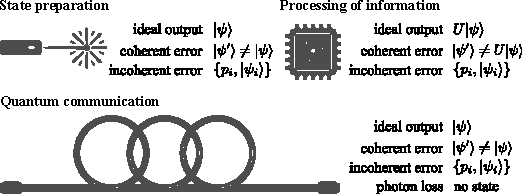
\includegraphics[width=\textwidth]{lesson3/3-1_noise.pdf}
    \caption[Noisy world]{Real quantum states are noisy.}
    \label{fig:3-1_noise}
\end{figure}

The last example deals with the central scenario of these lecture notes, namely \textbf{\emph{quantum communication}}\index{quantum communication}.
Consider the case where you prepare a state $|\psi\rangle$, which you would like to send to a friend through a long optical fiber.
Even though we do not process the prepared state in any way, optical fibers themselves are sources of noise.
The state received by your friend will be affected by coherent and incoherent errors.
On top of these, the state may even get lost and never arrive due to various processes such as absorption or scattering in the fiber.
Photon loss is a huge headache in quantum communication and we will discuss it in great detail in later chapters.





\section{Outer product}
\label{sec:3-2_outer_product}

We have seen in the previous chapter that the inner product of two vector states $|a\rangle$ and $|b\rangle$ is formed by transforming the first ket into a bra and then multiplying them together,
\begin{equation}
    \langle a | b\rangle = \begin{pmatrix} a_0^* & a_1^* \end{pmatrix} \begin{pmatrix} b_0 \\ b_1 \end{pmatrix} = a_0^* b_0 + a_1^* b_1.
\end{equation}
What happens when we change the order of multiplication?
Let's multiply the ket $|b\rangle$ from the right by the bra $\langle a|$,
\begin{equation}
    | b\rangle \langle a | = \begin{pmatrix} b_0 \\ b_1 \end{pmatrix} \begin{pmatrix} a_0^* & a_1^* \end{pmatrix} = \begin{pmatrix} a_0^*b_0 & a_1^*b_0 \\ a_0^*b_1 & a_1^*b_1 \end{pmatrix}.
\end{equation}
By changing the order of multiplication, we obtained a complex matrix.
The above product of a ket with a bra, $|b\rangle\langle a|$, is called an \textbf{\emph{outer product}}\index{outer product}. It is necessary in order to describe measurements as well as noisy quantum states.

In order to see what the action of an outer product on a state vector is, we will begin with a few simple examples.
Let's consider the following outer product, $|0\rangle\langle0|$.
The matrix representation of $|0\rangle\langle0|$ is
\begin{equation}
    |0\rangle\langle0| = \begin{pmatrix} 1 \\ 0 \end{pmatrix} \begin{pmatrix} 1 & 0 \end{pmatrix} = \begin{pmatrix} 1 & 0 \\ 0 & 0 \end{pmatrix}.
\end{equation}
We also know from basic vector algebra that matrices transform vectors into other vectors.
Let's apply our example outer product to a general qubit state vector $|\psi\rangle = \alpha|0\rangle + \beta|1\rangle$, where $|\alpha|^2+|\beta|^2=1$,
\begin{align}
    |0\rangle\langle0|\psi\rangle & = |0\rangle\langle0| \left( \alpha|0\rangle + \beta|1\rangle \right) \label{eq:projector_00}\\
    & = \alpha |0\rangle\underbrace{\langle0|0\rangle}_{=1} + \beta |0\rangle\underbrace{\langle0|1\rangle}_{=0} \nonumber\\
    & = \alpha|0\rangle. \nonumber
\end{align}
In the second line of Eq.~(\ref{eq:projector_00}), we used the fact that the inner product of a normalized vector with itself is unity, and the orthogonality property of kets $|0\rangle$ and $|1\rangle$.
We see that our example outer product induces an interesting transformation of the initial general single-qubit state vector $|\psi\rangle$.
It changes the initial state vector into $|0\rangle$, up to a complex constant $\alpha$.
We did not assume any particular values for the initial probability amplitudes $\alpha$ and $\beta$, meaning that any initial state vector, provided $\alpha\neq0$, is transformed into a vector proportional to $|0\rangle$.
We say that $|0\rangle\langle0|$ \textit{\textbf{projects}} onto the state $|0\rangle$, and that the outer product is an example of a \textbf{\emph{projector}}\index{projector}.
The only time $|0\rangle\langle0|$ does not project onto $|0\rangle$ is when the initial state is orthogonal to $|0\rangle$, that is, when the initial state is $|1\rangle$.

Let's have a quick look at the action of a different outer product, namely $|1\rangle\langle1|$.
In matrix form, we have
\begin{equation}
    |1\rangle\langle1| = \begin{pmatrix} 0 \\ 1 \end{pmatrix} \begin{pmatrix} 0 & 1 \end{pmatrix} = \begin{pmatrix} 0 & 0  \\ 0 & 1 \end{pmatrix}.
\end{equation}
Since $|0\rangle\langle0|$ projects onto the state $|0\rangle$, we expect that $|1\rangle\langle1|$ projects onto $|1\rangle$.
Let's confirm this by acting with $|1\rangle\langle1|$ on a general state vector $|\psi\rangle$,
\begin{align}
    |1\rangle\langle1|\psi\rangle & = |1\rangle\langle1| \left( \alpha|0\rangle + \beta|1\rangle \right) \label{eq:projector_11}\\
    & = \alpha |1\rangle\underbrace{\langle1|0\rangle}_{=0} + \beta |1\rangle\underbrace{\langle1|1\rangle}_{=1} \nonumber\\
    & = \beta|1\rangle. \nonumber
\end{align}
Indeed, $|1\rangle\langle1|$ does project onto the $|1\rangle$ state.

Recall from Sec.~\ref{sec:measurement} that measurement in the $Z$ basis of a general qubit $|\psi\rangle = \alpha |0\rangle + \beta |1\rangle$ has two possible outcomes.
Outcome +1 is obtained with probability $|\alpha|^2$ and the post-measurement state is $|0\rangle$.
We just saw that this post-measurement state is obtained after application of the projector $|0\rangle\langle0|$, up to a factor of $\alpha$.
Similarly, he -1 outcome of the measurement is obtained with probability $|\beta|^2$ by application of the projector $|1\rangle\langle1|$, up to a factor of $\beta$.
The post-measurement state is $|1\rangle$ resulting from the application of the projector $|1\rangle\langle1|$.
The outer products $|0\rangle\langle0|$ and $|1\rangle\langle1|$ capture the effect of \textbf{\emph{projective measurements}}\index{projective measurements}.
The different probabilities of the measurement outcomes can also be readily calculated.
The probabilities are simply the expectation values of the projectors,
\begin{align}
    \langle \psi | 0 \rangle \langle 0 | \psi \rangle & = \left( \alpha^*\langle0| + \beta^*\langle1| \right) |0\rangle\langle0| \left( \alpha |0\rangle + \beta |1\rangle \right) = |\alpha|^2, \\
    \langle \psi | 1 \rangle \langle 1 | \psi \rangle & = \left( \alpha^*\langle0| + \beta^*\langle1| \right) |1\rangle\langle1| \left( \alpha |0\rangle + \beta |1\rangle \right) = |\beta|^2.
\end{align}

Can you guess the form of the projectors corresponding to measurement in the Pauli $X$ basis?
We can follow the same logic that we have used for the case of $Z$-basis measurement.
Post-measurement state after a $\pm1$ outcomes is $|\pm\rangle$.
The corresponding projectors are
\begin{align}
    |+\rangle\langle+| & = \frac{1}{\sqrt{2}} \begin{pmatrix} 1 \\ 1 \end{pmatrix} \frac{1}{\sqrt{2}} \begin{pmatrix} 1 & 1 \end{pmatrix} = \frac{1}{2} \begin{pmatrix} 1 & 1 \\ 1 & 1 \end{pmatrix}, \\
    |-\rangle\langle-| & = \frac{1}{\sqrt{2}} \begin{pmatrix} 1 \\ -1 \end{pmatrix} \frac{1}{\sqrt{2}} \begin{pmatrix} 1 & -1 \end{pmatrix} = \frac{1}{2} \begin{pmatrix} 1 & -1 \\ -1 & 1 \end{pmatrix}.
\end{align}
We can also convince ourselves that these operators really do project onto the correct states by applying them to a general qubit state,
\begin{align}
    |+\rangle\langle+|\psi\rangle & = |+\rangle \frac{1}{\sqrt{2}} \left( \langle0| + \langle1| \right) \left( \alpha |0\rangle + \beta|1\rangle \right) = \frac{\alpha+\beta}{\sqrt{2}} |+\rangle, \\
    |-\rangle\langle-|\psi\rangle & = |-\rangle \frac{1}{\sqrt{2}} \left( \langle0| - \langle1| \right) \left( \alpha |0\rangle + \beta|1\rangle \right) = \frac{\alpha-\beta}{\sqrt{2}} |-\rangle.
\end{align}
Similarly, projectors corresponding to the $\pm1$ outcomes of a measurement in the Pauli Y basis are
\begin{align}
    |i\rangle\langle i| & = \frac{1}{\sqrt{2}} \begin{pmatrix} 1 \\ i \end{pmatrix} \frac{1}{\sqrt{2}} \begin{pmatrix} 1 & -i \end{pmatrix} = \frac{1}{2} \begin{pmatrix} 1 & -i \\ i & 1 \end{pmatrix}, \\
    |-i\rangle\langle-i| & = \frac{1}{\sqrt{2}} \begin{pmatrix} 1 \\ -i \end{pmatrix} \frac{1}{\sqrt{2}} \begin{pmatrix} 1 & i \end{pmatrix} = \frac{1}{2} \begin{pmatrix} 1 & i \\ -i & 1 \end{pmatrix}.
\end{align}
The action of these projectors can be verified by applying them to an arbitrary qubit state,
\begin{equation}
    |i\rangle\langle i|\psi\rangle = \frac{\alpha-i\beta}{\sqrt{2}} |i\rangle, \quad
    |-i\rangle\langle-i|\psi\rangle = \frac{\alpha+i\beta}{\sqrt{2}} |-i\rangle.
\end{equation}

Before moving on, it is worth settling on the notation regarding projectors.
Sometimes, rather than writing projectors as outer products, we denote them by a single letter.
Usual choice is $\Pi$, the capital Greek letter ``pi'',
\begin{equation}
    \Pi_{\pm}^B \equiv |b_{\pm}\rangle\langle b_{\pm}|,
\end{equation}
where $B$ denotes the basis in which we are measuring and $|b_{\pm}\rangle$ denote the two orthogonal state vectors corresponding to the two possible measurement outcomes $\pm1$.
Table~\ref{tab:3-2_projectors} contains all six projectors that we have so far encountered written in both the short notation as well as outer products.
\begin{table}[h]
    \setcellgapes{3pt}
    \setlength{\tabcolsep}{15pt}
    \renewcommand\theadfont{}
    \makegapedcells
    \centering
    \begin{tabular}{ccc}
        \hline
        & \textbf{+1 Outcome} & \textbf{-1 Outcome} \\
        \hline
        \thead{Pauli $X$ basis} & $\Pi^X_+=|+\rangle\langle+|$ & $\Pi^X_-=|-\rangle\langle-|$ \\
        \thead{Pauli $Y$ basis} & $\Pi^Y_+=|i\rangle\langle i|$ & $\Pi^Y_-=|-i\rangle\langle-i|$ \\
        \thead{Pauli $Z$ basis} & $\Pi^Z_+=|0\rangle\langle0|$ & $\Pi^Z_-=|1\rangle\langle1|$ \\
        \hline
    \end{tabular}
    \caption{Projectors onto the eigenstates of the Pauli matrices.}
    \label{tab:3-2_projectors}
\end{table}

We have represented quantum states in the form of vectors.
For example,
\begin{equation}
    |0\rangle = \begin{pmatrix} 1 \\ 0 \end{pmatrix}, \quad |+\rangle = \frac{1}{\sqrt{2}} \begin{pmatrix} 1 \\ 1 \end{pmatrix}, \quad |\psi\rangle = \begin{pmatrix} \alpha \\ \beta \end{pmatrix}.
    \label{eq:3-2_vectors}
\end{equation}
We have also seen that outer products can project onto these states.
This suggests that we can equally \textbf{\emph{represent quantum states as matrices}} as well written in the form of outer products.
For example, the states in Eq.~(\ref{eq:3-2_vectors}) can be written as projectors in the following way,
\begin{equation}
    |0\rangle\langle0| = \begin{pmatrix} 1 & 0 \\ 0 & 0 \end{pmatrix}, \quad |+\rangle\langle+| = \frac{1}{2} \begin{pmatrix} 1 & 1 \\ 1 & 1 \end{pmatrix}, \quad |\psi\rangle\langle\psi| = \begin{pmatrix} |\alpha^*| & \alpha\beta^* \\ \alpha^*\beta & |\beta|^2 \end{pmatrix}.
\end{equation}
The state vector $|\psi\rangle$ and the projector $|\psi\rangle\langle\psi|$ represent the same state of a physical system.
You might ask yourselves, why complicate things with outer product description of quantum states if vectors seem to work just fine?
The vector description is sufficient only for a limited number of cases when the quantum systems are not affected by any imperfections.
Such states are called \textbf{\emph{pure states}}\index{pure states}.
So far we have been working exclusively with pure states.
In order to describe more realistic quantum states, we have to resort to description that relies on the outer product, as we will see in the next Section.



\section{Density matrices}
\label{sec:3-3_density_matrices}

\begin{figure}[t]
    \centering
    \includegraphics[width=\textwidth]{lesson3/3-3_noisy_communication.pdf}
    \caption[Noisy quantum communication]{Ideal quantum input state becomes a probabilistic mixture at the output as a result of the noise introduced by the optical fiber.}
    \label{fig:3-3_noisy_communication}
\end{figure}

Let's consider the scenario of sending an ideal quantum state $|\psi\rangle$ through an optical fiber as shown in Fig.~\ref{fig:3-3_noisy_communication}.
The state of the quantum system inevitably changes as it travels through the optical fiber.
The fiber affects the state of the quantum system probabilistically.
The system remains unaffected with some probability, but also with some probability it suffers from unwanted transformations.
The incoherent output becomes a distribution of states $\{p_i, |\psi_i\rangle\}$.
With probability $p_i$ the output is described by the state vector $|\psi_i\rangle$.

How can we describe such an incoherent output mathematically?
The output is not a single state that we know can be represented by a vector, rather it is a probabilistic distribution of such states.
Therefore we cannot represent it as a superposition.
Superposition of various state vectors is still a state that represents perfect knowledge of the quantum system, which we do not have.
The correct way of describing the incoherent output in Fig.~\ref{fig:3-3_noisy_communication} is by using the outer product that we learned about in the previous section.
The output state is a projector $|\psi_i\rangle\langle\psi_i|$ with probability $p_i$, and the whole output state can be described as a sum of all such projectors,
\begin{equation}
    p_1 |\psi_1\rangle\langle\psi_1| + p_2 |\psi_2\rangle\langle\psi_2| + \ldots + p_n |\psi_n\rangle\langle\psi_n|.
    \label{eq:3-3_mixture}
\end{equation}
The state represented by the sum in Eq.~(\ref{eq:3-3_mixture}) is called a \textbf{\emph{mixed state}}\index{mixed state}.
It is important to remember is that the $p_i$'s are probabilities and therefore they must sum to unity, that is $\sum_{i=1}^n p_i=1$.

\begin{figure}[t]
    \centering
    \includegraphics[width=0.9\textwidth]{lesson3/3-3_bit_flip_channel.pdf}
    \caption[Bit-flip channel]{Bit-flip channel. Pauli $X$ is applied to the input with probability $p$. The input is unaffected with probability $1-p$.}
    \label{fig:3-3_bit_flip_channel}
\end{figure}
In order to illustrate this on a simple example, we consider the  \textbf{\emph{bit-flip channel}}\index{bit-flip channel}, depicted in Fig.~\ref{fig:3-3_bit_flip_channel}.
The input is some general state $|\psi\rangle$.
The input is either affected by a Pauli $X$ transformation with probability $p$, or it is transmitted without errors with probability $1-p$.
We will denote the output by the Greek letter $\rho$ (rho),
\begin{equation}
    \rho = (1-p) |\psi\rangle\langle\psi| + p X|\psi\rangle\langle\psi|X.
    \label{eq:3-3_bit_flip}
\end{equation}
Let's explore how this channel works by considering a few simple inputs.
When the input is $|\psi\rangle = |0\rangle$, the output is
\begin{equation}
    \rho = (1-p)|0\rangle\langle0| + p|1\rangle\langle1| = \begin{pmatrix} 1-p & 0 \\ 0 & p \end{pmatrix}.
\end{equation}
On the other hand, if the input is $|\psi\rangle=|1\rangle$, we get
\begin{equation}
    \rho = (1-p)|1\rangle\langle1| + p|0\rangle\langle0| = \begin{pmatrix} p & 0 \\ 0 & 1-p \end{pmatrix}
\end{equation}
as the output.

We know that the general state of a pure state of a qubit is $|\psi\rangle = \alpha|0\rangle + \beta|1\rangle$.
What is the general form of a mixed state?
We have seen it already in Eq.~(\ref{eq:3-3_mixture}),
\begin{equation}
    \rho = \sum_i p_i |\psi_i\rangle\langle\psi_i|.
    \label{eq:general_mixed_state}
\end{equation}
The representation for a state vector we have used so far is known as a ket, while this more general representation using a sum of outer products is called a \textbf{\emph{density matrix}}\index{density matrix}.
Note that the density matrix can describe both pure and mixed states, whereas the state vector can only describe pure states.
When all $p_i$ values vanish except for one, that is $\rho=\ketbra{\psi}{\psi}$, the state $\rho$ is pure.
On the other hand, if more than one $p_i$ is non-zero, the state $\rho$ is mixed.  (The \ket{\psi} is not restricted to a single computational basis state; it can be any superposition.  That is, \ket{\psi} is not restricted to a state like \ket{0} or \ket{1}; $\ket{\psi} = \ket{+}$ is valid too.)

We saw in the previous chapter that all vectors representing quantum states must be normalized.
What does this normalization condition look like when we write the state as a density matrix?
To answer this question, let's first define the \textit{\textbf{trace}} of a matrix $A$,
\begin{equation}
    \text{Tr} \{ A \} = \sum_i A_{ii},
\end{equation}
as the sum of all the diagonal elements.
For example,
\begin{equation}
    A = \begin{pmatrix} A_{11} & A_{12} & A_{13} \\ A_{21} & A_{22} & A_{23} \\ A_{31} & A_{32} & A_{33} \end{pmatrix}, \qquad \text{Tr} \{ A \} = A_{11} + A_{22} + A_{33}.
\end{equation}
Density matrix $\rho$ is normalized when $\text{Tr}\{\rho\}=1$.
Let's test this on a general pure state $|\psi\rangle = \alpha |0\rangle + \beta |1\rangle$.
The density matrix  corresponding to $|\psi\rangle$ is
\begin{equation}
    \rho = |\psi\rangle\langle\psi| = \begin{pmatrix} |\alpha|^2 & \alpha\beta^* \\ \alpha^*\beta & |\beta|^2 \end{pmatrix}.
\end{equation}
We see that $\text{Tr}\{\rho\} = |\alpha|^2 + |\beta|^2 = 1$ if the state is normalized.

Computing the trace of a general density matrix can be made straightforward by the following realization.
The action of a trace on an outer product is to swap the places of the bra and the ket, changing the outer product into an inner product,
\begin{equation}
    \text{Tr} \{|b\rangle\langle a|\} = \langle a|b\rangle.
\end{equation}
Therefore for any pure state $|\psi\rangle$, we have
\begin{equation}
    \text{Tr}\{|\psi\rangle\langle\psi|\} = \langle\psi|\psi\rangle=1.
\end{equation}
How about a general mixed state $\rho$ given by the Eq.~(\ref{eq:general_mixed_state})?
The calculation is very similar,
\begin{align}
    \text{Tr}\{\rho\} & = \text{Tr}\left\{\sum_i p_i |\psi_i\rangle\langle\psi_i|\right\} \\
    & = \sum_i p_i \text{Tr}\left\{ |\psi_i\rangle\langle\psi_i| \right\} \nonumber\\
    & =\sum_i p_i \underbrace{\langle\psi_i|\psi_i\rangle}_{=1} \nonumber\\
    & = \sum_i p_i \nonumber\\
    & = 1.
\end{align}

\begin{figure}[t]
    \centering
    % 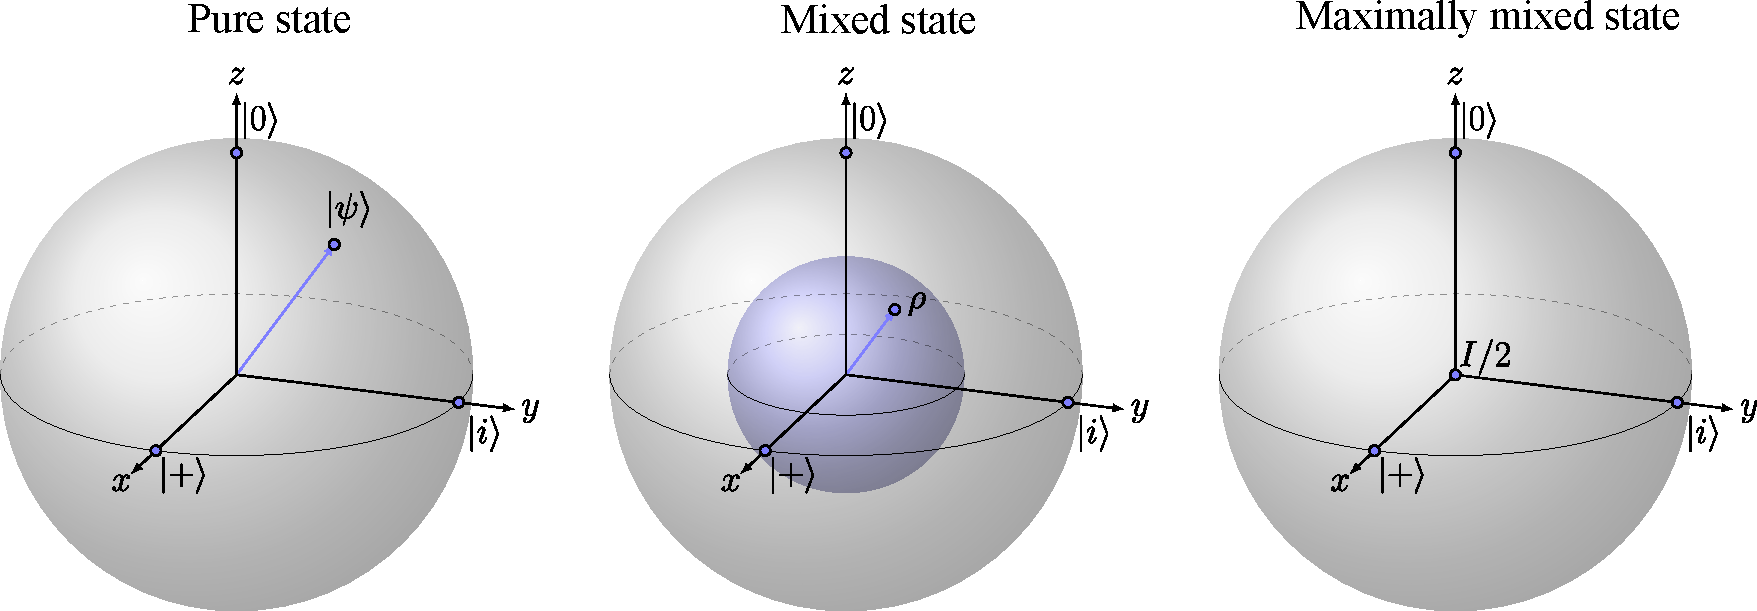
\includegraphics[width=\textwidth]{lesson3/3-3_bloch_new.pdf}
    \def\r{4}
    \tdplotsetmaincoords{70}{115}
    \def\azimuthP{40}
    \def\polarP{60}
    \def\circleSize{88.5}
    
    \begin{tikzpicture}[tdplot_main_coords,scale=0.35,every node/.style={scale=0.35}]

    \tdplotsetcoord{O}{0}{0}{0}
    \tdplotsetcoord{P}{\r}{\azimuthP}{\polarP}
    \tdplotsetcoord{Q}{\r*sin(\azimuthP)}{90}{\polarP}

    \shade[tdplot_screen_coords,ball color=gray!40,opacity=0.5] (0,0,0) circle (\r); 
    \tdplotCsDrawLonCircle[tdplotCsBack/.style={black!50,dashed},thin]{\r}{\polarP-90}
    \tdplotCsDrawLatCircle[tdplotCsBack/.style={black!50,dashed},very thin]{\r}{90-\azimuthP}
    \tdplotCsDrawLatCircle[tdplotCsBack/.style={black!50,dashed}]{\r}{0}

    \draw[-latex,semithick] (O) -- (1.3*\r,0,0) node[pos=1.15] {\Huge $x$};
    \draw[-latex,semithick] (O) -- (0,1.3*\r,0) node[pos=1.07] {\Huge $y$};
    \draw[-latex,semithick] (O) -- (0,0,1.3*\r) node[pos=1.06] {\Huge $z$};
    
    \draw[-latex,thick,blue!50] (O) -- (P);
    
    \tdplotCsDrawCircle[tdplotCsFill/.style=blue!50,thick]{\r}{\polarP}{\azimuthP}{1.05*\circleSize}
    \node[] at (4, 3.8, 5.1) {\Huge $|\psi\rangle$};
    \node[] at (0, 0, 6.5) {\Huge Pure state};

    \begin{scope}[xshift=10cm]
    
    \tdplotsetcoord{O}{0}{0}{0}
    \tdplotsetcoord{P}{0.4*\r}{\azimuthP}{\polarP}
    \tdplotsetcoord{Q}{0.4*\r*sin(\azimuthP)}{90}{\polarP}

    \shade[tdplot_screen_coords,ball color=gray!40,opacity=0.5] (0,0,0) circle (\r);
    \tdplotCsDrawLatCircle[tdplotCsBack/.style={black!50,dashed}]{\r}{0}

    \shade[tdplot_screen_coords,ball color=blue!30,opacity=0.5] (0,0,0) circle (0.4*\r);
    \tdplotCsDrawLonCircle[tdplotCsBack/.style={black!50,dashed},thin]{0.4*\r}{\polarP-90}
    \tdplotCsDrawLatCircle[tdplotCsBack/.style={black!50,dashed},thin]{0.4*\r}{90-\azimuthP}
    \tdplotCsDrawLatCircle[tdplotCsBack/.style={black!50,dashed}]{0.4*\r}{0}

    \draw[-latex,semithick] (O) -- (1.3*\r,0,0) node[pos=1.15] {\Huge $x$};
    \draw[-latex,semithick] (O) -- (0,1.3*\r,0) node[pos=1.07] {\Huge $y$};
    \draw[-latex,semithick] (O) -- (0,0,1.3*\r) node[pos=1.06] {\Huge $z$};
    
    \draw[-latex,thick,blue!50] (O) -- (P);
    
    \tdplotCsDrawCircle[tdplotCsFill/.style=blue!50,thick]{0.4*\r}{\polarP}{\azimuthP}{1.09*\circleSize}
    \node[] at (1, 1.8, 1.3) {\Huge $\rho$};
    \node[] at (0, 0, 6.5) {\Huge Mixed state};
    
    \end{scope}

    \begin{scope}[xshift=20cm]
    
    \tdplotsetcoord{O}{0}{0}{0}
    \tdplotsetcoord{P}{0.4*\r}{\azimuthP}{\polarP}
    \tdplotsetcoord{Q}{0.4*\r*sin(\azimuthP)}{90}{\polarP}

    \shade[tdplot_screen_coords,ball color=gray!40,opacity=0.5] (0,0,0) circle (\r);
    \tdplotCsDrawLatCircle[tdplotCsBack/.style={black!50,dashed}]{\r}{0}

    \draw[-latex,semithick] (O) -- (1.3*\r,0,0) node[pos=1.15] {\Huge $x$};
    \draw[-latex,semithick] (O) -- (0,1.3*\r,0) node[pos=1.07] {\Huge $y$};
    \draw[-latex,semithick] (O) -- (0,0,1.3*\r) node[pos=1.06] {\Huge $z$};

    \filldraw[blue!50,draw=black,thick] (0,0) circle (5pt);
    \node[] at (1, 1.5, 1.2) {\Huge $I/2$};
    \node[] at (0, 0, 6.5) {\Huge Maximally mixed state};
    
    \end{scope}  
    \end{tikzpicture}

    \caption[Bloch sphere and mixed states]{Bloch sphere representation of a pure state $|\psi\rangle$, a mixed state $\rho$ and the maximally mixed state $I/2$.}
    \label{fig:3-3_bloch}
\end{figure}

Mixed states can be visualized using the Bloch sphere as well.
Pure states are represented by the points on the surface of the sphere.
Mixed states, on the other hand, are represented by all the points \textbf{\emph{inside the Bloch sphere}}, as shown in Fig.~\ref{fig:3-3_bloch}.
The closer we get to the centre of the sphere, the more mixed the quantum state becomes.
The center of the sphere is where the \textbf{\emph{maximally mixed state}}\index{maximally mixed state},
\begin{equation}
    \frac{1}{2} |0\rangle\langle0| + \frac{1}{2} |1\rangle\langle1| = \frac{1}{2} \begin{pmatrix} 1 & 0 \\ 0 & 1 \end{pmatrix} = \frac{I}{2},
\end{equation}
is located.
This point represents zero knowledge about the quantum state.
If we measure this state in the Pauli $Z$ basis, both outcomes are equally likely.
We can think about this state as being ``half-way between'' the pure states $|0\rangle$ and $|1\rangle$.
However, there is nothing sacred about the Pauli $Z$ basis.
We can also think about the maximally mixed state being ``half-way between'' the pure states $|+\rangle$ and $|-\rangle$, and write it as
\begin{equation}
    \frac{I}{2} = \frac{1}{2} |+\rangle\langle+| + \frac{1}{2} |-\rangle\langle-|.
\end{equation}
This immediately suggests that if we measure the maximally mixed state in the Pauli $X$ basis then both outcomes are equally likely again.
You may have guessed that we can also use the Pauli $Y$ basis and write the maximally mixed state as $I/2 = ( |i\rangle\langle i| + |-i\rangle\langle-i| ) / 2$.






%%%%%%%%%%%%%%%%%%%%%%%%%%%%%%%%%%%%%%%%%%%%%%%%%%%%
\section{Pure vs mixed states}
\label{sec:3-4_pure_vs_mixed}

Now that we have seen how pure and mixed states differ in terms of their representations, it is a good time to pause and consider the difference between them.
We mentioned that pure states represent states of full knowledge whereas mixed states are necessary if there is some uncertainty about the quantum state.
How can we see this difference in real life when we do measurements?
Let's consider two quantum states, one is an equal superposition of $|0\rangle$ and $|1\rangle$, and the other is an equal mixture of $|0\rangle$ and $|1\rangle$,
\begin{align}
    |\psi\rangle & = \frac{1}{\sqrt{2}} (|0\rangle + |1\rangle, \label{eq:3-4_superposition}\\
    \rho & = \frac{1}{2} (|0\rangle\langle0| + |1\rangle\langle1|). \label{eq:3-4_mixture}
\end{align}
We can immediately see that when we measure both states in the Pauli $Z$ basis, we obtain the same statistics for the measurement outcomes,
\begin{align}
    \text{superposition} \; |\psi\rangle & : \text{Prob}\{+1\} = \text{Prob}\{-1\} = \frac{1}{2},  \\
    \text{mixture} \; \rho & : \text{Prob}\{+1\} = \text{Prob}\{-1\} = \frac{1}{2}.
\end{align}
This means that we cannot tell these two states from each other by performing just a Pauli $Z$ measurement.
It also seems to go counter to our intuition that pure states represent full knowledge of the state. After all, we cannot predict the outcome of a measurement with certainty.
We will see that this is not quite true.

Let's measure the two states again but this time in the Pauli $X$ basis.
We can rewrite the two states in Eq.~(\ref{eq:3-4_superposition})-(\ref{eq:3-4_mixture}) in the Pauli $X$ basis,
\begin{align}
    |\psi\rangle & = |+\rangle, \\
    \rho & = \frac{1}{2} (|+\rangle\langle+| + |-\rangle\langle-|).
\end{align}
Probabilities of the measurement outcomes are now very different,
\begin{align}
    \text{superposition} \; |\psi\rangle & : \text{Prob}\{+1\} = 1, \; \text{Prob}\{-1\} = 0,  \\
    \text{mixture} \; \rho & : \text{Prob}\{+1\} = \text{Prob}\{-1\} = \frac{1}{2}.
\end{align}
We see that measuring the superposition $|\psi\rangle$ in the Pauli $X$ basis always results in a positive measurement outcome.
On the other hand, when measuring the mixture, both outcomes are still equally likely.
We can see that the equal superposition and equal mixture can be distinguished from each other when measured in the Pauli $X$ basis.
Now the meaning of having perfect knowledge of the states becomes more clear.
The outcome of measuring this state in the $X$ basis is deterministic: it always gives the same outcome. More generally, for any pure state, there is always some choice of measurement we could make that will give a deterministic outcome. For mixed states, on the other hand, the measurement outcomes in any basis will always be probabilistic.

The above procedure allows us to tell pure states from mixed states, but it is rather complicated.
We have to check the measurement statistics for various bases, which can be quite laborious.
Fortunately, there is a very simple way of checking if a state $\rho$ is pure or mixed using the \textbf{\emph{purity}}\index{purity} $\gamma$, pronounced ``gamma''.
Purity is defined as the trace of the square of the density matrix,
\begin{equation}
    \gamma = \text{Tr} \{ \rho^2 \} \longrightarrow \begin{cases}
        = 1, \quad \text{when } \rho \text{ is pure}, \\
        < 1, \quad \text{when } \rho \text{ is mixed}.
    \end{cases}
\end{equation}
When the quantum state is pure, the purity is $\gamma=1$.
On the other hand, when the state is mixed, purity is strictly less than 1.

\begin{table}[t]
    \setcellgapes{5pt}
    \renewcommand\theadfont{}
    \makegapedcells
    \centering
    \begin{tabular}{ccc}
        \hline
        & \textbf{Pure states} & \textbf{Mixed states} \\
        \hline
        Notation & $|\psi\rangle$ & $\rho$ \\
        Represented by & vectors or matrices & matrices only \\
        Normalization & $\langle\psi|\psi\rangle=1$ & $\text{Tr}\{\rho\}=1$ \\
        Knowledge of the state & perfect & imperfect \\
        Purity & 1 & $<1$ \\
        \hline
    \end{tabular}
    \caption[Pure versus mixed states]{Summary of differences between pure and mixed states.}
    \label{tab:3-4_pure_vs_mixed}
\end{table}

This brings our discussion of the differences between pure and mixed states to an end.
Table~\ref{tab:3-4_pure_vs_mixed} provides a summary of the important points.




\section{Fidelity}
\label{sec:3-5_fidelity}

One thing you should always keep in mind is that it is impossible to exactly prepare the desires pure state.
Sometimes the prepared state is pure but not quite the target state we were aiming for.
Other times it can be affected by incoherent noise resulting in a mixed state.
It is crucial that we have a way of quantifying the difference between the real and the desired, or target, state.

A convenient tool that tells us how close the real state is to the target state is the \textbf{\emph{fidelity}}\index{fidelity}.
Consider the case where the target state is a pure state $|\psi\rangle$.
This state could be the desired output of a quantum computer, or a state distributed by a quantum network.
However, due to noise and imperfections in the hardware and our control of it, the actual state is inevitably some mixture $\rho$.
The deviation of this state from the target state is given by the fidelity $F$, defined as
\begin{equation}
    F(\rho,|\psi\rangle) = \langle\psi|\rho|\psi\rangle.
    \label{eq:3-5_fidelity}
\end{equation}
Note that other more general definitions for fidelity are sometimes used as well, particularly when the target state is not pure but mixed.
However, we will only consider scenarios where the target state is pure and therefore Eq.~(\ref{eq:3-5_fidelity}) will be sufficient.

Let's consider the case where the real state is equal to the target state, $\rho=|\psi\rangle\langle\psi|$.
The fidelity is then
\begin{equation}
    F(\rho,|\psi\rangle) = \bra{\psi}\rho\ket{\psi} = \underbrace{\langle\psi|\psi\rangle}_{=1} \underbrace{\langle\psi|\psi\rangle}_{=1} = 1.
\end{equation}
On the other hand, when the real state $|\phi\rangle$ is pure but orthogonal to the target state,
\begin{equation}
    F(\rho,|\psi\rangle) = \langle\psi|\rho|\psi\rangle = \underbrace{\langle\psi|\phi\rangle}_{=0} \underbrace{\langle\phi|\psi\rangle}_{=0} = 0.
\end{equation}
Orthogonal states are as far from each other as can be and this is signified by a vanishing fidelity.
In fact, the two cases considered above are the two extreme ones, and for general mixed state,
\begin{equation}
    0 \leq F(\rho,|\psi\rangle) \leq 1.
\end{equation}

Let's continue with another example.
Consider the case where we would like to prepare the state $|0\rangle$, but something goes very wrong with our hardware and the real state that we obtain after the preparation procedure is the maximally mixed state $\rho = (|0\rangle\langle0| + |1\rangle\langle1|)/2$.
The fidelity can be computed as follows,
\begin{align}
    F(\rho,|0\rangle) & = \langle 0 | \left[\frac{1}{2}(|0\rangle\langle0| + |1\rangle\langle1|)\right] | 0 \rangle \nonumber\\
    & = \frac{1}{2} \underbrace{\langle0|0\rangle}_{=1} \underbrace{\langle0|0\rangle}_{=1} + \frac{1}{2} \underbrace{\langle0|1\rangle}_{=0} \underbrace{\langle1|0\rangle}_{=0} \nonumber\\
    & = \frac{1}{2}.
\end{align}
It is interesting to note that the fidelity does not vanish.
We said that the maximally mixed state is where we have maximum uncertainty whether it is \ket{0} or \ket{1}, yet the fidelity with a pure state only drops to a half.

We can extend this example to two qubits and consider the fidelity between the pure target state $|00\rangle$ and the maximally mixed state $\rho = (|00\rangle\langle00|+|01\rangle\langle01|+|10\rangle\langle10|+|11\rangle\langle11|)/4=I/4$,
\begin{equation}
    F(\rho, |00\rangle) = \langle00| \rho | 00\rangle = \frac{1}{4} \langle 00| I |00\rangle = \frac{1}{4}.
\end{equation}
This calculation can be quickly extended to $N$ qubits.
The fidelity between the state $|0\rangle^{\otimes N}$ and a maximally mixed state of $N$ qubits, given by $\rho=I/2^N$.
The fidelity is
\begin{equation}
    F(\rho,|0\rangle^{\otimes N}) = \frac{1}{2^N}.
\end{equation}
We see that the fidelity scales with the number of qubits but never quite reaches zero.

As our last example, we will consider the bit-flip channel of Eq.~(\ref{eq:3-3_bit_flip}).
Let's again consider the initial state to be $|0\rangle$ and compute how the fidelity changes depending on the probability of error $p$.
We have
\begin{align}
    F(\rho,|\psi\rangle) & = \langle0| \rho | 0\rangle \\
    & = \langle0| \left[ (1-p)|0\rangle\langle0| + p|1\rangle\langle1| \right] |0\rangle \nonumber\\
    & = (1-p) \langle0|0\rangle \langle0|0\rangle + p \langle0|1\rangle \langle1|0\rangle \nonumber\\
    & = 1 - p.
\end{align}
The fidelity does depend on the probability of error, as we anticipated.
When $p=0$, meaning there is no bit-flip noise affecting the input state, the fidelity of the output state is 1.
On the other hand, if the bit-flip channel is maximally noisy, $p=1/2$, the output state is the maximally mixed state.
This is also evidenced by the fidelity dropping to $F(\rho,|0\rangle)=1/2$.

We mentioned that the fidelity is an important tool in quantifying the quality of a quantum state with respect to the ideal noiseless case.
It can be interpreted as the probability that real state is the target state.
Many protocols in quantum communication as well as quantum computation do not work when the real state is too noisy.
Often this condition is expressed in the form of a \textbf{\emph{threshold fidelity}}\index{threshold fidelity} $F_{crit}$.
If the fidelity of the real state is above this critical value, $F > F_{crit}$, then the protocol can be successfully executed.
On the other hand, if $F < F_{crit}$, the protocol cannot be used.
An example of such a protocol is entanglement purification, where the fidelity of noisy entangled pairs can be boosted provided the initial pairs are not too noisy.
Another example is fault-tolerant quantum computation, where scalable universal quantum computation can be achieved even with noisy components, provided the noise is below a certain threshold.


\newpage
\begin{exercises}

\exer{
\label{ex:dirac-notation-measurement}
\emph{Single-qubit measurements}.
Consider a general pure state $|\psi\rangle=\alpha|+\rangle+\beta|-\rangle$. Calculate the probabilities $\text{Pr}\{+1\}$ and $\text{Pr}\{-1\}$ in the following cases:
\subexer{
When the state is measured in the $X$ basis.
}
\subexer{
When the state is measured in the $Y$ basis.
}
\subexer{
When the state is measured in the $Z$ basis.
}
% \subexer{One way to find the post-measurement state of a state is
% $$\ket{\psi'} = \frac{M_i\ket{\psi}}{\sqrt{\bra{\psi} M_i\ket{\psi}}}$$ when the outcome is $i$. Show that this gives exactly \ket{0} or \ket{1} when measuring in the computational basis, when $\ket{\psi} = \alpha\ket{0}+\beta\ket{1}$, for any valid values of $\alpha$ and $\beta$.
% }
}

\exer{
\emph{Post-measurement state.} We have seen in Section~\ref{sec:3-2_outer_product} that a projector transforms the initial state into a state that resembles the expected state after the measurement. In order to obtain the correct post-measurement state $|\psi'\rangle$, we have to renormalize by the square root of the probability of the measurement outcome,
\begin{equation*}
    |\psi'\rangle = \frac{\Pi^B_i|\psi\rangle}{\sqrt{\langle\psi|\Pi^B_i|\psi\rangle}},
\end{equation*}
where index $i\in\{+1,-1\}$ denotes the measurement outcome. Obtain the post-measurement states in the following scenarios:
\subexer{
Initial state is $|\psi\rangle=\alpha|0\rangle + \beta|1\rangle$, it is measured in the $Z$ basis, the outcome is +1.
}
\subexer{
Initial state is $|\psi\rangle=|0\rangle$, it is measured in the $Y$ basis, the outcome is -1.
}
\subexer{
Initial state is $|\psi\rangle=|+\rangle$, the state is measured in the $X$ basis, can we obtain the -1 outcome?
}
}

\exer{
\emph{Mixed states}. We have a quantum machine that prepares a particular quantum state. By using our machine many times, we have determined that 60\% of the time, the machine prepares the state $|0\rangle$, 20\% of the time, it prepares the state $|1\rangle$, and 20\% of the time, it prepares the state $|+\rangle$.
\subexer{
Write down the state the machine prepares using Dirac notation.
}
\subexer{
What is the matrix representation of this state?
}
}

\exer{
\emph{Maximally mixed state}. We have seen that, considered in the Z basis, the density matrix for a completely mixed state of a single qubit has $1/2$ in each of the two entries on the diagonal,
\begin{equation*}
    \rho=\left(\begin{array}{cc}
    1/2 & 0 \\
    0 & 1/2
    \end{array}\right).
\end{equation*}
\subexer{
Prove that when measuring $\rho$ in the $X$ basis, the probability of finding each outcome is also $1/2$.
}
\subexer{
Prove that a completely mixed state of $\ket{+}$ and $\ket{-}$ is equal to the fully mixed state of $\ket{0}$ and $\ket{1}$.
}
}

\exer{
\emph{Bit-flip channel}. We have introduced the bit-flip channel,
\begin{equation}
    \rho = (1-p)|\psi\rangle\langle\psi| + p X|\psi\rangle\langle\psi|X,
\end{equation}
where an initial pure state $|\psi\rangle$ is transformed into a final mixed state by a probabilistic application of the Pauli $X$ operator.
}

\end{exercises}

